\section{Laboratory work implementation}

\subsection{Tasks and Points}
\begin{itemize}
\item \textbf{Basic Level (grade 5 - 6) you should be able to:}
	\begin{enumerate}
	\item Create an animation based on Windows timer which involves at least 5 different drawn objects
      \end{enumerate}
\item \textbf{Normal Level (grade 7 - 8) you should be able to:}
      \begin{enumerate}
    \item Realize the tasks from \textit{Basic Level}.
    \item Increase and decrease animation speed using mouse wheel/from keebord
    \item Solve flicking problem describe in your readme/report the way you had implemented this
          \end{enumerate}
\item \textbf{Advanced Level (grade 9 - 10) you should be able to:}
      \begin{enumerate}
    \item Add 2 animated objects which will interact with each other. Balls that have different velocity and moving angles. They should behave based on following rules::
    	\begin{enumerate}
        \item At the begining you should have 3 bals of different colours of the same size
        \item On interaction with each other, if they are of the same class (circle, square), they shuld change their color and be multiplied.
        \item On interaction with the right and left wall (the margins of the window), they should be transformed into squares.
        \item On interaction with the top and bottom of the window - the figures should increase their velocity.
        \item Please, take into consideration that the user can increase and decrease animation speed using mouse wheel/from keebord
        \end{enumerate}
          \end{enumerate}
\item \textbf{for Bonus Point Tasks :}
\begin{enumerate}
	\item For the task above, add balls with mouse.
    \end{enumerate}
  \end{itemize}  

\clearpage
\subsection{Prove your work with screens}



\begin{figure}[h!]
  \centering
    {%
      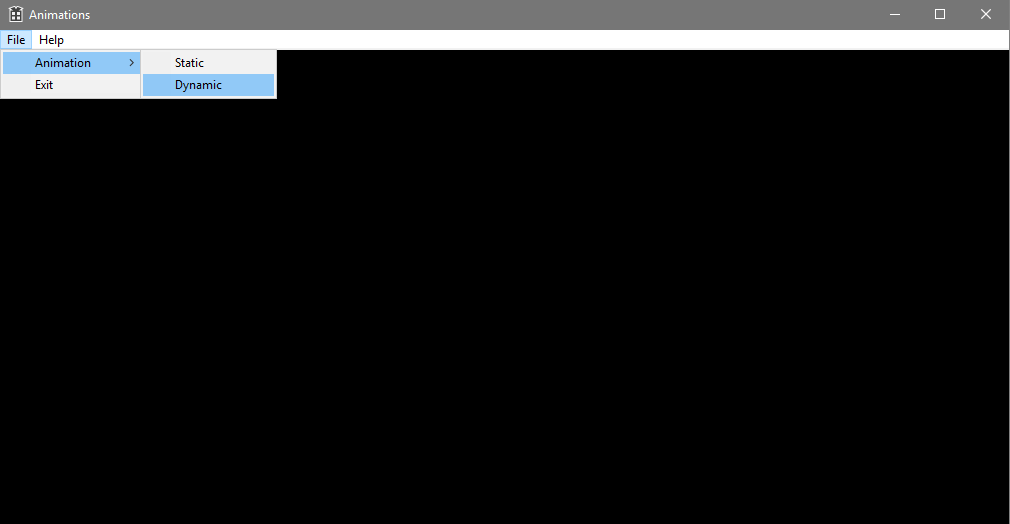
\includegraphics[width=1\textwidth]{1}}
  \caption{There are 2 options in menu first one which is "Static" is for first task to create 5 animated different objects , the obj changes their size but do not move.}
\end{figure}

\begin{figure}[h!]
  \centering
    {%
      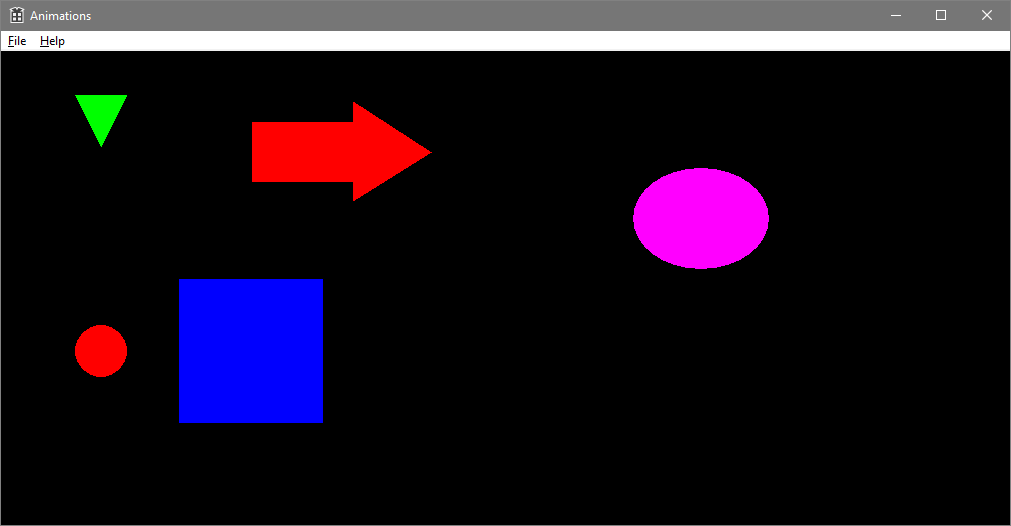
\includegraphics[width=1\textwidth]{2}}
  \caption{Animation of static option from menu.}
\end{figure}

\begin{figure}[h!]
  \centering
    {%
      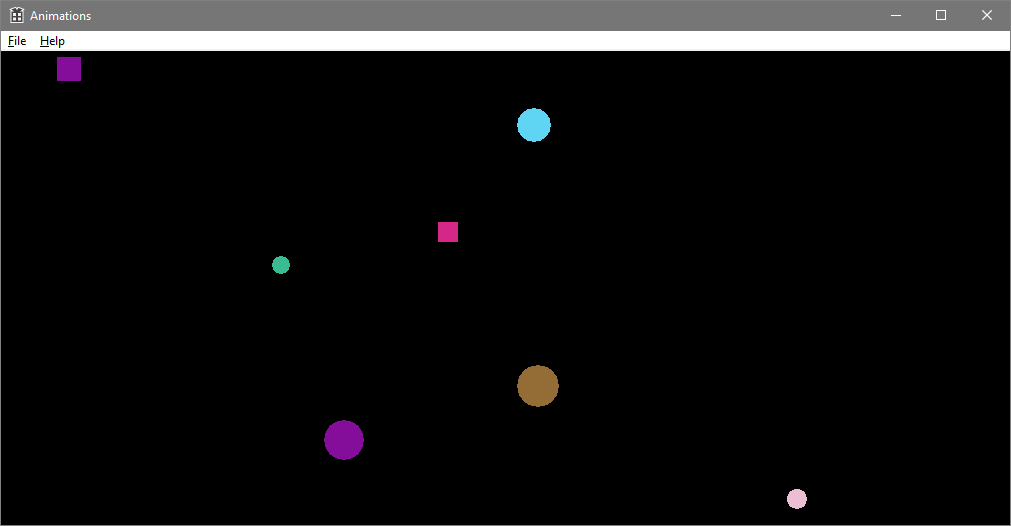
\includegraphics[width=1\textwidth]{3}}
  \caption{Animation of dynamic option from menu.}
\end{figure}

 